\documentclass[a4paper,10pt,numbers=noendperiod]{scrartcl}
\setlength\oddsidemargin{0.2cm}
\setlength\evensidemargin{0.2cm}
\setlength\textwidth{15.8cm}

\usepackage{amsfonts}
\usepackage{amssymb}
\usepackage{amsmath}
\usepackage{amsthm}
\usepackage{tikz}
\usepackage{wasysym}
\usepackage{ucs}
\usepackage{stmaryrd}
\usepackage{hyperref}
\usepackage{graphicx}
\usepackage{nicefrac}
\usepackage[english]{babel}
%\usepackage{marvosym}
\usepackage{dsfont}
\usepackage{listings}
\usepackage[utf8x]{inputenc}
\usepackage[T1]{fontenc}
\usepackage{enumitem}
\usepackage{tabularx}
\usepackage{url}
\usepackage{eurosym}

%\def\thesubsubsection{Exercise \arabic{section}.\alph{subsection}.\arabic{subsubsection}} 
%\def\thesubsection{\arabic{section}.\alph{subsection} - } 
%\def\thesection{\arabic{section}}



\lstset{ %
language=C++,                % the language of the code
basicstyle=\footnotesize,       % the size of the fonts that are used for the code
numbers=left,                   % where to put the line-numbers
numberstyle=\footnotesize,      % the size of the fonts that are used for the line-numbers
stepnumber=1,                   % the step between two line-numbers. If it's 1, each line 
numbersep=5pt,                  % how far the line-numbers are from the code
backgroundcolor=\color{white},  % choose the background color. You must add \usepackage{color}
showspaces=false,               % show spaces adding particular underscores
showstringspaces=false,         % underline spaces within strings
showtabs=false,                 % show tabs within strings adding particular underscores
frame=single,                   % adds a frame around the code
tabsize=2,                      % sets default tabsize to 2 spaces
captionpos=b,                   % sets the caption-position to bottom
breaklines=true,                % sets automatic line breaking
breakatwhitespace=false,        % sets if automatic breaks should only happen at whitespace
title=\lstname,                 % show the filename of files included with \lstinputlisting;
}



\author{Ralph Krimmel}
\title{xmpproxy, a proxy server for the XMPP protocol}
\subtitle{ Project description and plan }


\begin{document}
\maketitle{}
\thispagestyle{empty}
\newpage
\tableofcontents{}
\newpage
\section{Abstract}
\textit{``The extensible messaging and presence protocol xmpp is an open technology 
for real time communication which powers a wide range of applications including instant messaging, 
presence, multi-party chat, voice and video calls, collaboration, lightweight middleware, 
content syndication and generalized routing of xml data.''}   $_{\tiny http://xmpp.org/about}$ \\

Being widely used in several large communication platforms such as \texttt{Google talk},  % Todo cite
\texttt{XMPP} has become an important protocol for communication via network. This document will describe an 
issue using \texttt{XMPP}'s instant messaging capabilities in a multi client environment and propose a possible solution.
It also contains a time schedule for implementing this solution as a project for the course ``Applied IT project'' at the University 
of Gothenburg.

\section{Introduction}
The \texttt{XMPP} or ``jabber''-protocol supports multiple clients to be connected to the same account at the same time. From the server sides view a connected client is called a \textit{ressource}. The consequence of multiple ressources for the same account is that the server has to decide to which ressource an incoming message, or \textit{stanza} in xmpp terminology, is routed to. This is done via the so called \textit{presence priority} a client can connect with.  The client with the higher priority will receive the message. 
If two or more ressources have the same priority, the server may use some other rule to decide between those or deliver the message to all of them. For example, the server could use the most recent connect time or the most recent activity time. However, the server is not allowed to deliver the stanza to an available resource with a negative priority. %TODO cite 

This behaviour leads to the problem, that conversations and logfiles of conversations may not be complete on every client, if one client connects with a higher priority. Figure \ref{fig:2clients} shows an example where this would be the case. Client A does not know the parts of the conversation that are held from Client B. Also, not just incoming messages will be missing, Client A will not even know about outgoing stanzas from Client B. 
\begin{figure}[h!]
	\begin{center}
		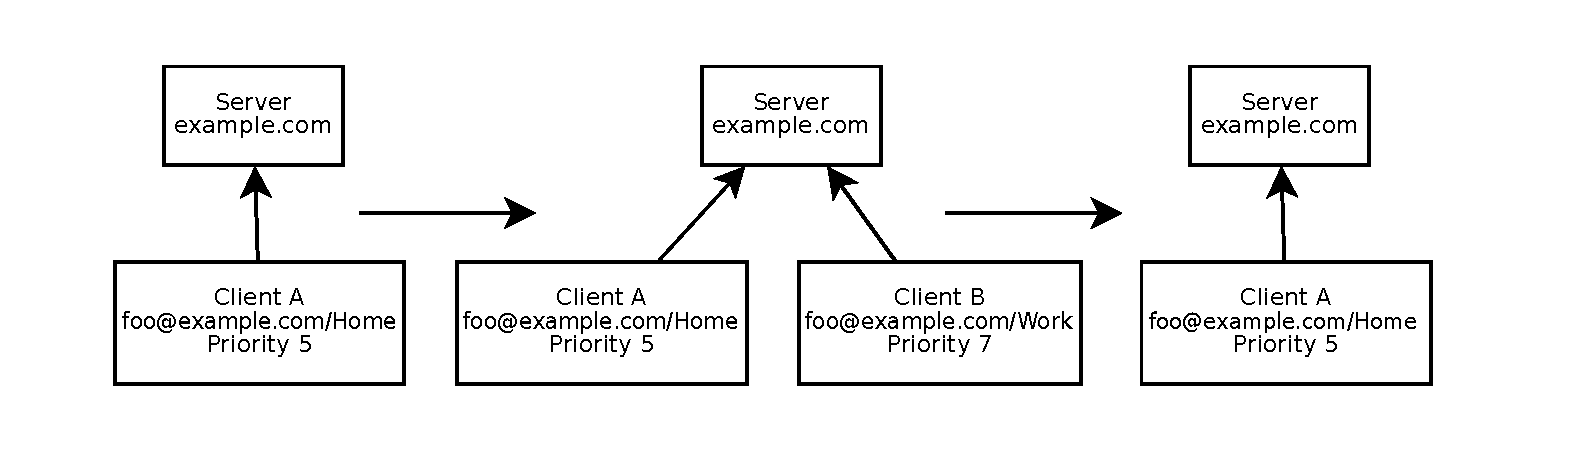
\includegraphics[scale=0.6]{figures/diagram1.pdf}
	\end{center}
	\caption{Clients with 2 different priorities are connected to the same account.}
	\label{fig:2clients}
\end{figure}


A possible solution for this issue may be the use of a proxy server as it can be seen in figure \ref{fig:2clientsproxy}. This server will make sure, that every incoming stanza will reach both clients and every outgoing stanza will be sent to every ressource as well as to the targeted server.

\begin{figure}[h!]
	\begin{center}
		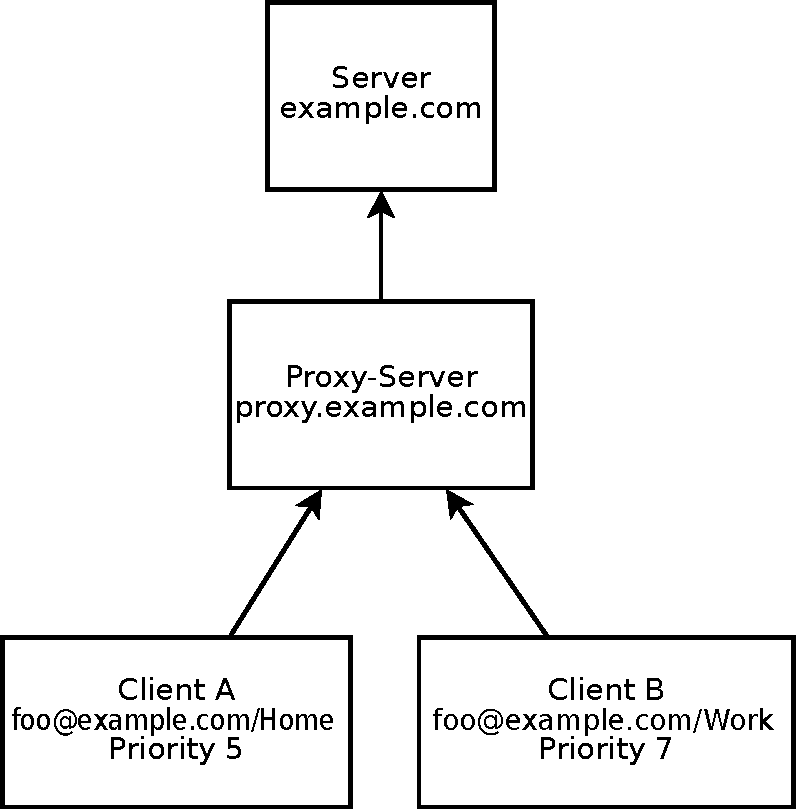
\includegraphics[scale=0.4]{figures/diagram3.pdf}
	\end{center}
	\caption{Two clients connected to a proxy.}
	\label{fig:2clientsproxy}
\end{figure}

\section{Technology}
\subsection{Software choice}
For implementing the xmpp proxy server several design descisions had to me made. First of all a programming language was chosen. Possible languages were Perl, C, C++ and Java because of the preferences of the author. The criteria for the programming language was first of all the availability of proper libraries that deal with the xmpp protocol, both server and client side.  Unfortunately, this excluded all languages except perl because there are just few xmpp server libraries at all. Therefore the xmpp proxy server will make use of the \texttt{djabberd} xmpp/jabber server and the perl modules \texttt{Net::XMPP/Net::XMPP::Client} although it lacks a proper documentation.
\subsection{Djabberd}
Djabberd is a modular, scalable and extensible jabber server written in perl where almost everything defers to hooks to be implemented by plugins. %cite
It is written and maintained by \textit{Brad Fitzpatrick}, \textit{Artur Bergman} and \textit{Jonathan Steinert}.
When this document was created, the most recent version of djabberd was 0.85, released on the thirteenth of June in 2011. Having a modular structure, djabberd is a perfect framework for building the required proxy server because it offers hooks for modifying the behaviour of the authentication and authorization process, roster storage and message delivery. Also, \texttt{djabberd} can be used in environments which require a high performance for it is asynchrone/event-based, using epoll on linux 2.6.

\subsection{Net::XMPP}
\texttt{Net::XMPP} is a perl package that provides access to XMPP client side functions for the perl programming language. It is maintaned by \textit{Eric Hacker} and versioned 1.02 at the time this document was written.
It can be utilized using its object oriented interface. 
There are objects available which hold the actual client functions like login, wait for messages, send messages and logout. 
Also there are objects for storing and handling Jabber IDs (\texttt{Net::XMPP::JID}), messages (\texttt{Net::XMPP::Message}), presence information (\texttt{Net::XMPP::Presence}) and Info/Query namespaces (\texttt{Net::XMPP::IQ}).  

\section{Tasks}
The following tasks are to be completed:
\begin{itemize}
	\item Studies of literature
	\item Write and test wrapper classes for djabberd and Net::XMPP data structures 
	\item Write and test module for proxy authentication
	\item Write and test module for proxy roster handling
	\item Write and test module for proxy presence handling 
	\item Write and test module for message delivery 
	\item (Optional) Write and test module for proxy groupchat
	\item (Optional) Write and test module for proxy jingle (Voice/Video via jabber)	
	\item Write Documentation	
	\item Write Report
	\item Create presentation
\end{itemize}


\section{Schedule}
The xmpproxy software will be written in the context of the course ``Applied IT Project'' course at the University of Gothenburg. This requires to ``formulate and execute a finite Applied IT project within a limited time-frame''. 
Therefore it is neccessary to schedule the tasks described in the previous sections. 
Table \ref{tab:estimatedtime} shows the percentage of effort and the estimated time every task will take. The minimum amoount of time this project will need is about 200 hours.


\begin{table}[h]
	\centering
	\begin{tabular}{|l|c|c|}
	\hline
	\textbf{Task} & \textbf{Percentage} & \textbf{Estimated time (in h)} \\
	\hline
	\hline
	Studies of literature & 10 & 20 \\
	\hline
	Wrapper classes for djabberd and Net::XMPP data structures & 4 & 8 \\
	Testing & 1 & 2\\
	\hline
	Module for proxy authentication & 4 & 8 \\
	Testing & 1 & 2 \\
	\hline
	Module for proxy roster handling & 8 & 16 \\ 
	Testing & 2 & 4 \\ 
	\hline
	Module for proxy presence handling & 8 & 16 \\ 
	Testing & 2 & 4 \\ 
	\hline
	Write module for message delivery & 16 & 32 \\
	Testing & 4 & 8\\
	\hline
	Documentation & 15 & 30\\
	\hline
        Report & 15 & 30\\
	\hline
	Presentation & 10 & 20\\
	\hline
	(Optional) Module for proxy groupchat & - & \\
	\hline
	(Optional) Module for proxy jingle (Voice/Video via jabber) & - & \\
	\hline
	\end{tabular}
	\caption{Estimated time for several tasks}
	\label{tab:estimatedtime}
\end{table}


\section{Literature}
\begin{itemize}
	\item \texttt{Programming jabber - extending XML messaging} by DJ Adams\\
	\item \url{http://xmpp.org/rfcs/rfc6120.html}\\
	\item \url{http://xmpp.org/rfcs/rfc6121.html}\\
	\item \url{http://xmpp.org/rfcs/rfc6122.html}\\
	\item \url{http://search.cpan.org/~hacker/Net-XMPP-1.02/}\\
	\item \url{http://search.cpan.org/~mart/DJabberd-0.85/}\\
\end{itemize}


\end{document} 
